% Overleaf-ready short-paper draft.
% IMPORTANT: Confirm the author list, author order, and affiliations with every
% contributor before any external submission.  The current author block names
% the repository owner/requester only; earlier team work is credited in the
% text and bibliography without assigning undocumented individual roles.
\documentclass[10pt,twocolumn]{article}

\usepackage[letterpaper,margin=0.72in]{geometry}
\usepackage{amsmath,amssymb,amsthm}
\usepackage{booktabs}
\usepackage{graphicx}
\usepackage{microtype}
\usepackage{xcolor}
\usepackage{url}
\usepackage[hidelinks]{hyperref}

\setlength{\columnsep}{0.23in}
\setlength{\emergencystretch}{2em}

\newtheorem{proposition}{Proposition}
\newcommand{\Z}{\mathbb{Z}}
\newcommand{\TV}{\operatorname{TV}}
\newcommand{\Lz}{L_0}

\title{Fiber Cancellation Creates a QFT Certification Gap\\
in Finite Regev-Style Factoring}
\author{Summer Malik\\
University of North Carolina at Charlotte\\
\small Short-paper draft for collaborator review}
\date{July 2026}

\begin{document}
\maketitle

\begin{abstract}
Distance-truncated quantum Fourier transforms (QFTs) remove small controlled
rotations, but a safe transform-level error bound can be much more demanding
than a factoring algorithm's actual needs.  We audit one such bound in a
finite Regev-style pipeline and prove that it cannot certify any non-exact
cutoff when $M<4\pi dm/\Delta$.  This is a limitation of the certificate, not
a lower bound on useful Fourier precision.  Modular-exponentiation fibers can
cancel coherent phase error before measurement, and an explicit finite case
has the same exact and truncated measurement law although the certificate
rejects.  We then freeze eight small semiprimes, two exact finite input-state
models, three Fourier moduli, all cutoffs, and a complete
sample-to-augmented-lattice-to-LLL-to-factor endpoint.  The certificate allows
zero omitted layers, whereas one omitted layer meets a preregistered
10-percentage-point non-inferiority rule in all six model--modulus cells; two
layers pass for the finite-Gaussian model at $M=16,32$.  The largest passing
cutoff removes six logical controlled phases and twelve QFT-only transpiled
CX gates.  These results establish a finite, model- and decoder-specific
certification gap, not asymptotic approximate-QFT sufficiency or end-to-end
hardware speedup.
\end{abstract}

\section{Introduction}

Shor's algorithm made integer factoring a central application of quantum
period finding~\cite{Shor1994,Shor1997}.  Regev later proposed a factoring
algorithm that reduces the quantum gate count per circuit, under a
number-theoretic conjecture, by using multidimensional Fourier samples and
more substantial classical lattice reduction~\cite{Regev2025}.  This trade
raises a practical precision question: must every controlled phase in each
Fourier register be retained for the downstream lattice decoder to work?

Approximate QFTs are not new.  Prior work analyzes truncated or banded QFTs
inside factoring and period-finding algorithms, including their task-level
success rather than only matrix error~\cite{Coppersmith1994,BarencoEtAl1996,
FowlerHollenberg2004,NamBlumel2012,NamBlumel2013}.  We therefore ask a narrow
question specific to the audited repository:

\begin{quote}
Does rejection by a conservative, all-input QFT certificate imply loss at a
finite multidimensional Regev-style lattice-and-factor endpoint?
\end{quote}

Our falsifiable hypothesis was that the certificate is conservative because
it discards the modular-fiber and measurement structure of the prepared
state.  The study makes four bounded contributions.

\begin{enumerate}
\item It gives a line-by-line audit and exact scaling limitation for the
implemented worst-case certificate.
\item It identifies arithmetic-fiber cancellation as a mechanism and provides
an equal-measurement-law counterexample to the implication ``certificate
rejection means information loss.''
\item It evaluates every cutoff in a frozen eight-modulus holdout using a
complete exact-lattice/LLL/stored-root factor endpoint, with the modulus---not
repeated shot batches---as the unit of generalization.
\item It records a pre-holdout QFT-ordering correction, sharper finite
factor-blind diagnostics, raw data, seeds, and resource counts.
\end{enumerate}

The result is a \emph{certification gap}: some rejected cutoffs tolerate a
bounded empirical recovery loss in the tested regime.  The truncated pipeline
does not outperform exact-QFT recovery, and we do not claim a new QFT
synthesis, a proof for full Regev sampling, or quantum advantage.

\paragraph{Implementation lineage.}
A companion artifact by Amorim, Barnes, and Malik developed an exact classical
simulator for the uniform exponent-box Fourier law, retained the prime roots
associated with squared circuit bases, implemented exact-rational LLL
post-processing, and introduced a uniform-sample null control
\cite{AmorimBarnesMalik2026}.  It has no finite-Gaussian input or approximate
QFT circuit, so it is an engineering and methodological predecessor rather
than evidence for the truncation claim here.  The present repository adds the
circuit audit, immutable root provenance, explicit $L$ versus $\Lz$
classification, finite-Gaussian model, QFT interventions and certificates,
and frozen held-out evaluation~\cite{Malik2026Artifact}.

\section{Finite Regev-style endpoint}

\subsection{Roots, squared bases, and useful relations}

Let $N$ be an odd composite, and choose units $b_1,\ldots,b_d\pmod N$ without
using the factors of $N$.  The circuit bases are the paired residues
\begin{equation}
  a_i=b_i^2\pmod N.
\end{equation}
The implementation stores every pair $(b_i,a_i)$ immutably.  This is necessary
because a residue can have several modular square roots; factor extraction
must use the root that generated the circuit base, not an arbitrary square
root reconstructed later.

Define the arithmetic map and two relation lattices
\begin{align}
 h_A(x)&=\prod_{i=1}^{d}a_i^{x_i}\pmod N,\\
 L&=\left\{z\in\Z^d:\prod_i a_i^{z_i}=1\pmod N\right\},\\
 \Lz&=\left\{z\in L:\prod_i b_i^{z_i}\in\{1,-1\}\pmod N\right\}.
\end{align}
For $z\in L$, let $\beta(z)=\prod_i b_i^{z_i}\bmod N$.  Then
$\beta(z)^2=1\bmod N$.  A vector in $\Lz$ is a valid but non-factor-yielding
relation.  A vector in $L\setminus\Lz$ gives a nontrivial square root of one;
the endpoint tests $\gcd(\beta-1,N)$ and $\gcd(\beta+1,N)$.  It first verifies
membership in $L$ and performs this classification without known factors or
group orders.

\subsection{Exact finite sampling law}

Let $M=2^q$, $[M]=\{0,\ldots,M-1\}$, and let
$g(x)=\prod_i w(x_i)$ be a separable real amplitude.  Before the product
inverse QFT, the normalized joint state is
\begin{equation}
 |\psi_w\rangle=\frac{1}{\sqrt Z}\sum_{x\in[M]^d}
 g(x)|x\rangle|h_A(x)\rangle,
 \qquad Z=\sum_x |g(x)|^2.
\end{equation}
After tracing out the arithmetic register, the exact finite measurement law
for a cutoff-$t$ inverse QFT $F_{M,t}^{-1}$ is
\begin{equation}
 P^{(t)}_{A,w}(k)=\frac{1}{Z}\sum_y\left|
 \sum_{x:h_A(x)=y}g(x)
 \langle k|(F_{M,t}^{-1})^{\otimes d}|x\rangle
 \right|^2. \label{eq:fiber-law}
\end{equation}
For the exact transform,
$\langle k|F_M^{-1}|x\rangle=M^{-1/2}e^{-2\pi i kx/M}$.
Equation~\eqref{eq:fiber-law} exposes the roots-of-unity sums inside each
arithmetic fiber $\{x:h_A(x)=y\}$.

We evaluate two finite laws exactly up to floating-point roundoff.  Model A is
the notebook's uniform hard box, $w(j)=1$.  Model B uses centered truncated discrete-Gaussian
amplitudes $w(j)=\exp(-\pi z_j^2/R^2)$ with
$z_j\in[-M/2,M/2)$ and $R=4$.  Model B is closer to Regev's state, but remains
a small finite simulation rather than his asymptotic parameter regime.

\subsection{Samples to an exact integer lattice}

Given $m$ measured rows $k_j\in[M]^d$, place them in
$K\in\Z^{m\times d}$ and set $W=K/M$.  With scale $S$, the augmented lattice
is generated by the columns of
\begin{equation}
 B=\begin{bmatrix}I_d&0\\SW&SI_m\end{bmatrix}.
\end{equation}
If $S=p_s/r_s$ in lowest terms, the code reduces the exactly cleared integer
row basis
\begin{equation}
 \mathcal A=(r_s M B)^\mathsf{T}=
 \begin{bmatrix}r_sMI_d&p_sK^\mathsf{T}\\0&p_sMI_m\end{bmatrix}.
 \label{eq:augmented}
\end{equation}
SymPy's exact integer LLL transform~\cite{LenstraLenstraLovasz1982} exposes
the candidate $z$ in its first $d$ transformation coefficients.  The primary
endpoint scans the Gram--Schmidt prefix specified by Regev's recovery
argument, verifies $z\in L$, tests $z\in\Lz$ using stored roots, and finally
attempts the two gcds.  No bounded enumeration, BKZ, quotient deflation, or
known-factor oracle is used in the frozen endpoint.

\section{Worst-case certificate and its gap}

Cutoff $t\in\{0,\ldots,q-1\}$ retains controlled phases whose qubit
separation is at most $t$; $t=q-1$ is exact.  At separation $r$, a $q$-qubit
QFT has $q-r$ phases of angle $\pi/2^r$.  Thus the omitted-angle tail is
\begin{equation}
 \eta(q,t)=\pi\sum_{r=t+1}^{q-1}\frac{q-r}{2^r}.
 \label{eq:eta}
\end{equation}

\begin{proposition}[Audited certificate limitation]
For $d$ Fourier registers, $m$ independent executions, and allowed absolute
event-probability change $0<\Delta<1$, the implemented certificate approves a
cutoff only if
\begin{equation}
 \min\!\left(1,m\min(1,2d\eta(q,t))\right)\leq\Delta.
 \label{eq:cert}
\end{equation}
Consequently,
\begin{equation}
 M<\frac{4\pi dm}{\Delta}
 \quad\Longrightarrow\quad
 \text{no non-exact cutoff is approved.} \label{eq:barrier}
\end{equation}
\end{proposition}

\begin{proof}
A controlled phase obeys
$\|\mathrm{CP}(\theta)-I\|_2=2|\sin(\theta/2)|\leq|\theta|$.
Telescoping the omitted gates gives
$\|F_M-F_{M,t}\|_2\leq\eta(q,t)$; telescoping the $d$ tensor factors gives
$\|F_M^{\otimes d}-F_{M,t}^{\otimes d}\|_2\leq d\eta(q,t)$.
The conservative pure-state-to-measurement step yields one-shot
$\TV\leq\min(1,2d\eta)$.  Replacing one coordinate at a time in the
$m$-sample product law gives Eq.~\eqref{eq:cert}, and every downstream event
differs by at most this TV distance.  The least aggressive non-exact cutoff is
$t=q-2$, for which $\eta(q,q-2)=2\pi/M$.  Substitution, clipping, and
$\Delta<1$ give the strict implication in Eq.~\eqref{eq:barrier}.
\end{proof}

These inequalities are standard operator, data-processing, and hybrid
bounds; we do not claim them as new.  Their audited composition explains why
the finite selector refuses all savings.  For the frozen
$d=2,m=7,\Delta=0.05$ experiment, the right side of the threshold is about
$3518.6$, far above every tested $M\leq32$.

\subsection{Why rejection does not imply information loss}

The operator norm maximizes over all input states, while
Eq.~\eqref{eq:fiber-law} restricts amplitudes to modular fibers and then
measures.  Omitted phases can cancel within a fiber, alter only low-mass
outcomes, or rotate amplitudes without changing their squared sums.  For
$N=15$, squared bases $(4,1)$, $d=2$, $M=4$, and $t=0$, direct finite fiber
summation gives identical exact and truncated measured laws (numerical
$\TV=5.9\times10^{-35}$), although Eq.~\eqref{eq:cert} rejects.  This
deliberately degenerate counterexample refutes a logical implication; it is
not a broad factoring benchmark.

Three factor-blind finite refinements diagnose the gap: exact measured-law
TV with an $m$-sample hybrid, exact product-Hellinger composition, and trace
distance on the prepared joint fiber state.  They are exponentially expensive
in $M^d$ and are validation tools, not scalable replacements for Regev's
analysis.  In the proof-slack audit, the median omitted-gate triangle factor is
$1.18$, while the median state-to-measurement factor is $6.80$.  A separate
$M=128$ example nearly saturates the first gate step (ratio $0.9998996$),
locating the important conservatism after the gate-level bound.

\paragraph{Implementation correction.}
Before the holdout, matrix tests found that the custom approximate inverse QFT
iterated qubits in the reverse gate order.  The previous full-cutoff test had
silently substituted a library QFT and therefore missed the error.  The
implementation was corrected so that retaining every phase reproduces the
direct roots-of-unity matrix; sign, swaps, endianness, layer order, and each
cutoff now have regression tests.  Every pre-correction approximate-QFT row
was invalidated and regenerated, and none enters this study.

\section{Frozen experiment}

The protocol was committed before the result manifest.  It fixed roots
$(2,3)$ and their squared bases, $d=2$, $M\in\{8,16,32\}$, $m=7$, both models,
every valid cutoff, $S=4$, relation bound $T=4$, LLL parameter $3/4$, 64
coupled replicates per cell, and master seed \texttt{2026071301}.  Exact and
approximate trials share seeds.  The eight held-out semiprimes were
\begin{equation*}
 55,\ 65,\ 85,\ 95,\ 115,\ 119,\ 133,\ 161.
\end{equation*}
No modulus was excluded.  Their known factors were used only after recovery
to validate a returned pair; state construction, certificates, LLL, relation
classification, and cutoff selection never receive them.

For each $N$, success probability is estimated over the 64 paired replicates.
Inference resamples the eight whole-$N$ clusters 5,000 times.  A cutoff is
declared empirically non-inferior only when the 95\% lower confidence bounds
for both factor recovery and verified $L\setminus\Lz$ recovery are at least
$-0.10$ relative to exact QFT.  This ten-percentage-point engineering margin
was frozen independently of the theorem's stricter $\Delta=0.05$ certificate
budget.  It is not an information-theoretic guarantee.

The experiment contains 192 per-$N$ configurations and 12,288 raw trials.
Its two primary outcomes are factor recovery and recovery of at least one
verified $L\setminus\Lz$ relation.  These outcomes coincide in the selected
cells because every recovered nontrivial stored-root class yielded the
verified factor pair; this is observed, not assumed for arbitrary composites.

\section{Results}

The original certificate approved zero omitted layers in all six
model--modulus cells.  One omitted layer met the frozen non-inferiority rule in
all six cells.  Two layers passed only for finite-Gaussian Model B at
$M=16,32$.  Table~\ref{tab:results} reports the largest passing omission in
each cell.  All recovery differences are approximate minus exact, and the
means average the eight per-$N$ probabilities.

\begin{table*}[t]
\centering
\caption{Largest omission meeting the frozen rule.  CI denotes the 95\%
whole-$N$ cluster-bootstrap interval.  Gate counts cover only the two product
QFT blocks.}
\label{tab:results}
\scriptsize
\begin{tabular}{ccrrrrrrr}
\toprule
$M$ & Model & Layers omitted & Exact mean & Approx. mean & Difference & 95\% CI & CP saved & CX saved\\
\midrule
8  & A & 1 & 0.1191 & 0.1074 & $-0.0117$ & $[-0.0273,\ 0]$       & 2 & 4\\
8  & B & 1 & 0.0898 & 0.0879 & $-0.0020$ & $[-0.0117,\ 0.0059]$  & 2 & 4\\
16 & A & 1 & 0.1699 & 0.1641 & $-0.0059$ & $[-0.0137,\ 0]$       & 2 & 4\\
16 & B & 2 & 0.0840 & 0.0469 & $-0.0371$ & $[-0.0742,\ 0]$       & 6 & 12\\
32 & A & 1 & 0.1992 & 0.1934 & $-0.0059$ & $[-0.0176,\ 0]$       & 2 & 4\\
32 & B & 2 & 0.0703 & 0.0527 & $-0.0176$ & $[-0.0352,\ -0.0039]$ & 6 & 12\\
\bottomrule
\end{tabular}
\end{table*}

\begin{figure*}[t]
\centering
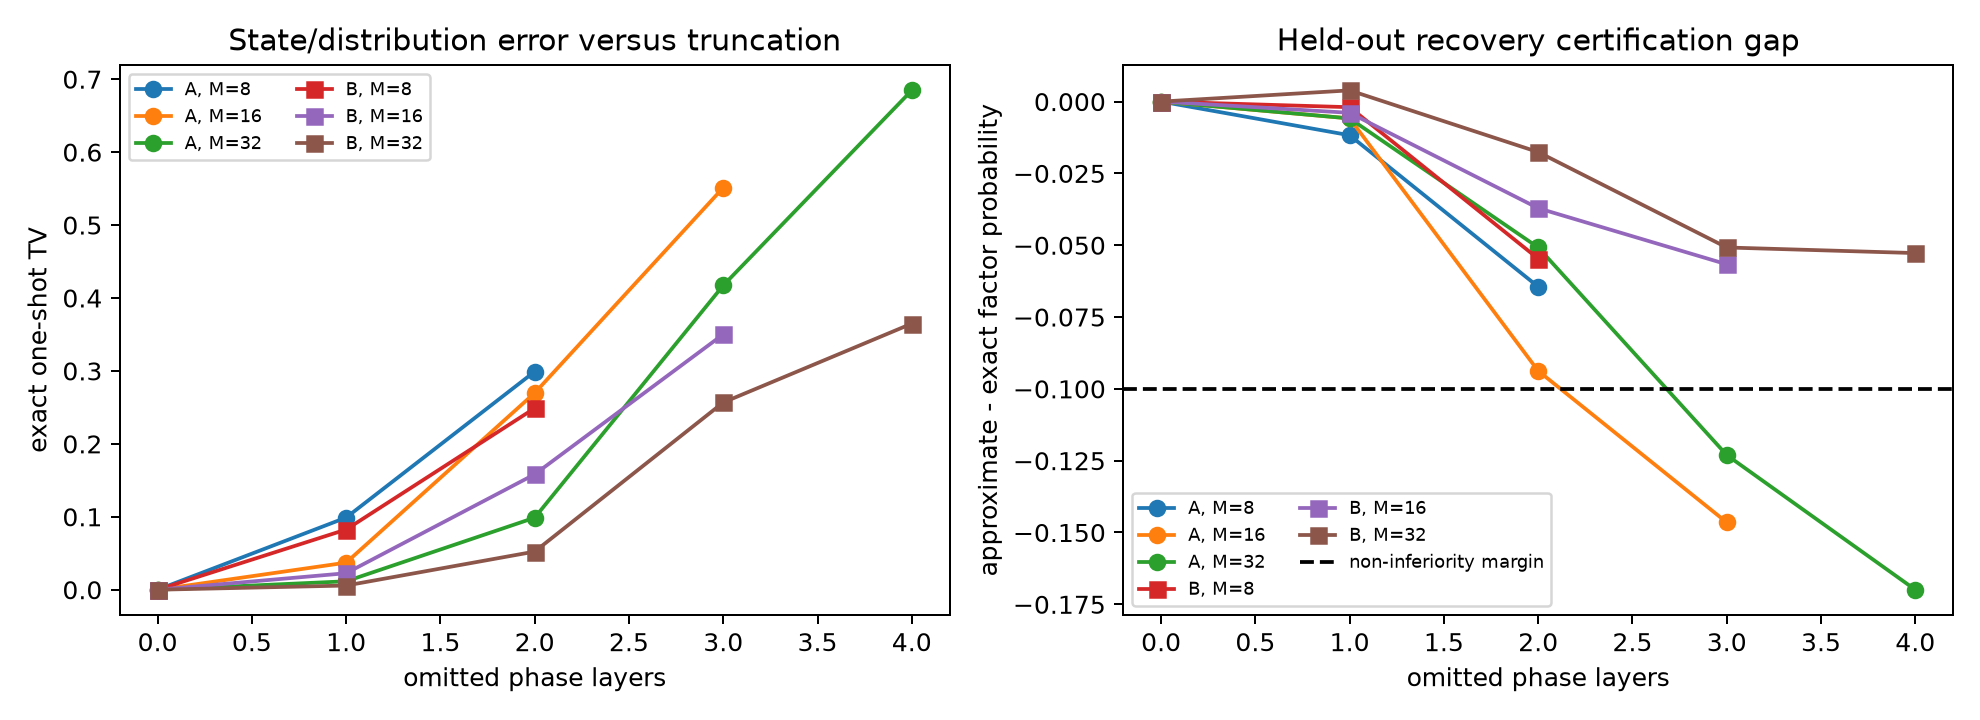
\includegraphics[width=0.96\textwidth]{figures/certification_vs_recovery.png}
\caption{Left: exact one-shot distribution TV versus omitted layers for the
representative modulus $N=55$ only.  Right: paired factor-probability
differences aggregated across all eight held-out $N$ values; the dashed line
is the frozen $-0.10$ margin.  Passing cutoffs lie above that line after the
confidence-bound test, not merely by their plotted mean.}
\label{fig:gap}
\end{figure*}

The approximate pipeline does not improve recovery; it accepts a measured
loss in exchange for fewer QFT gates.  More aggressive cutoffs fail in most
cells, so the result is not ``truncation never matters.''  The largest passing
cutoff removes six logical controlled phases and twelve QFT-only transpiled
CX gates.  Depending on the cell, QFT-only depth savings range from zero to
four.  Modular arithmetic is not included and may dominate full-circuit
depth, so these are not hardware-runtime or end-to-end savings.

Post-hoc margin sensitivity preserves at least one layer in all six cells at
a $0.05$ margin, but two layers remain only for Gaussian $M=32$.  At $0.02$,
hard-box $M=8$ permits no omission.  Thus the strongest ``one layer in every
cell'' statement depends on tolerating more than two percentage points of
absolute loss.  Leave-one-$N$-out checks retain the primary decisions but do
not create new held-out data.

A representative sharper-certificate row illustrates the mechanism.  For
$N=55$, Model B, $M=32$, and one omitted layer, one-shot TV is $0.005748$;
the seven-shot TV and Hellinger bounds are $0.04024$ and $0.03955$,
respectively.  Both are below $\Delta=0.05$ although the all-input certificate
rejects.  These finite refinements close only part of the empirical gap: the
two-layer Gaussian cells are not uniformly certified across held-out moduli.

\section{Prior-art boundary and limitations}

Task-aware approximate-QFT evaluation is established in Shor-style period
finding~\cite{Coppersmith1994,BarencoEtAl1996,FowlerHollenberg2004,
NamBlumel2012,NamBlumel2013}; our claim is limited to the specified
multidimensional sampler and exact Regev-style lattice endpoint.  Recent work
also studies implementations of Regev factoring~\cite{PawlitkoEtAl2026} and
noise-robust post-processing under a structured fraction of corrupted circuit
executions~\cite{RagavanVaikuntanathan2026}.  Coherent QFT truncation changes
every run's distribution and is not automatically covered by the latter
sparse-corruption model.

The holdout is small and structurally narrow: every $N$ is a small semiprime
containing factor 5 or 7.  We test only $d=2$, roots $(2,3)$, $M\leq32$,
$m=7$, $R=4$, ideal finite A/B laws, one distance-based truncation, and one
LLL decoder.  Model A is a notebook surrogate.  Model B is a truncated finite
Gaussian, not a proof-level realization of Regev's asymptotic state.  There
is no gate-level hardware noise, calibrated device run, cryptographic-scale
instance, full modular-arithmetic resource comparison, or proof that every
postprocessor preserves recovery.  With only eight $N$ clusters, confidence
intervals are necessarily coarse, and the frozen $0.10$ margin is a design
choice rather than a universal scientific threshold.

The exact state and finite certificate calculations scale exponentially in
$M^d$.  They certify and explain toy instances; they do not dequantize Regev's
algorithm in the complexity-theoretic sense.  A scalable theorem exploiting
fiber structure while bounding the complete lattice event remains open.

\section{Conclusion}

The experiments and audit support three separately scoped claims.

\paragraph{Verified implementation correction.}
The custom approximate-QFT order was wrong, the masking test was replaced,
and all affected results were regenerated before evaluation.

\paragraph{Verified finite empirical result.}
For the frozen eight-semiprime A/B study and current LLL endpoint, the
worst-case certificate allows zero truncation while the cutoffs in
Table~\ref{tab:results} meet the declared recovery-loss criterion and save
QFT-local gates.

\paragraph{Unverified general hypothesis.}
Arithmetic-fiber-aware reasoning may enable scalable precision selection for
larger Regev instances.  The present data do not establish that claim.

The practical lesson is modest but important: failure of a sufficient
all-state certificate is not evidence of algorithmic or information-theoretic
failure.  Precision decisions should retain the structure of the prepared
state, its measurement, and the actual classical endpoint whenever that
structure can be analyzed.

\section*{Artifact and reproducibility}

The accompanying archive contains this source, bibliography, frozen
configuration, selected raw summary tables, the plotted figure, checksums, and
a verification script.  The complete code and all 12,288 trial rows are in
the research repository at commit
\texttt{a4a47c77aa9e5935597d9a3c37fc6efe9f8b1d04}
\cite{Malik2026Artifact}.  The primary reproduction entry point is
\texttt{scripts/run\_qft\_certificate\_gap.py}.

\paragraph{Authorship note.}
The author block is provisional.  Before external circulation or submission,
the collaborators should confirm authorship, author order, affiliations, and
which results may be publicly attributed.

\bibliographystyle{unsrt}
\bibliography{references}

\end{document}
